%基礎電気回路理論
\chapter{基礎電気回路理論}


本書では、電磁気学の基礎法則から出発し、
電気回路としてそれらがどのように表現されるかを学んできた。
本章では、回路理論の要点を整理し、各概念の関係をまとめる。

\section{電圧・電流・回路素子}

回路理論では、主に電圧 $V$、電流 $I$、電荷 $Q$ を基本量として扱う。

\begin{itemize}
\item 電流は電荷の時間変化として定義される
\begin{equation}
I = \frac{dQ}{dt}
\end{equation}

\item 電圧はエネルギーの差を表す量であり、
電場の線積分として定義される
\begin{equation}
V = -\int \vec{E} \cdot d\vec{l}
\end{equation}
\end{itemize}

これらの量を結びつける要素として、
抵抗、コンデンサ、コイルが導入される。



\section{基本回路素子}

\subsection{抵抗}

抵抗は電流と電圧を比例関係で結ぶ素子であり、
オームの法則に従う。

\begin{equation}
V = RI
\end{equation}

抵抗はエネルギーを熱として消費する散逸素子である。



\subsection{コンデンサ}

コンデンサは電荷を蓄える素子であり、
電圧と電荷の関係は

\begin{equation}
Q = CV
\end{equation}

で表される。
エネルギーは電場として蓄えられる。



\subsection{コイル}

コイルは電流の変化に対して起電力を生じる素子であり、

\begin{equation}
V = L\frac{dI}{dt}
\end{equation}

で表される。
エネルギーは磁場として蓄えられる。



\section{キルヒホッフの法則}

回路全体の振る舞いは、以下の二つの法則によって記述される。

\begin{itemize}
\item 電流則（KCL）：節点における電流の保存
\begin{equation}
\sum I = 0
\end{equation}

\item 電圧則（KVL）：閉回路におけるエネルギー保存
\begin{equation}
\sum V = 0
\end{equation}
\end{itemize}

これらは、それぞれ電荷保存則とエネルギー保存則に基づいている。



\section{時間応答と過渡現象}

RC回路やRL回路では、
回路量は時間に依存して変化し、指数関数的な応答を示す。

\begin{equation}
e^{-t/\tau}
\end{equation}

で表される時定数 $\tau$ は、
回路の応答速度を決定する重要な指標である。



\section{交流回路とインピーダンス}

交流回路では、電圧と電流は時間的に変動するため、
複素数表示を用いた解析が有効である。

各素子のインピーダンスは

\begin{align}
Z_R &= R \\
Z_L &= j\omega L \\
Z_C &= \frac{1}{j\omega C}
\end{align}

で定義され、
直列回路では単純に加算される。



\section{電磁気学とのつながり}

回路理論は電磁気学の近似として理解できる。

\begin{itemize}
\item 電圧：電場の線積分
\item 電流：電荷の流れ
\item インダクタンス：電磁誘導
\item コンデンサ：電場エネルギー
\end{itemize}

特にキルヒホッフの法則は、
マクスウェル方程式を回路スケールで近似した結果とみなせる。

\section{その他重要な知識}
\subsection{抵抗分圧}

直列に接続された抵抗に電圧を加えると、
各抵抗にかかる電圧は抵抗値に比例して分配される。
これを抵抗分圧という。


\begin{figure}[h]
    \centering
    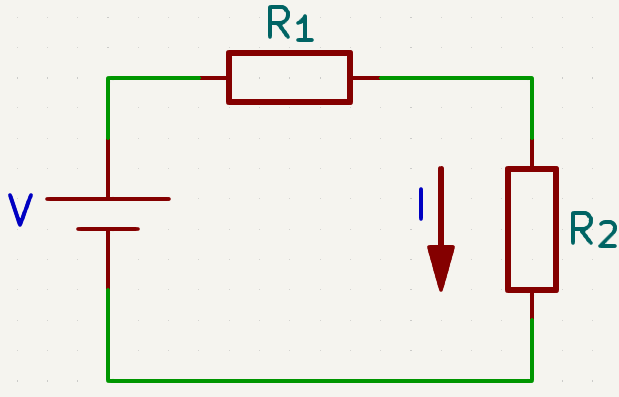
\includegraphics[width=0.5\textwidth]{circuit_theory/voltage_divider.png}
    \caption{抵抗分圧回路の例}
    \label{fig:voltage_divider}
\end{figure}

\subsection{分圧の式}

直列回路では電流は共通であり、

\begin{equation}
I = \frac{V_{\mathrm{in}}}{R_1 + R_2}
\end{equation}

である。

抵抗 $R_2$ にかかる電圧（出力電圧）は

\begin{align}
V_{\mathrm{out}}
&= I R_2 \\
&= \frac{R_2}{R_1 + R_2} V_{\mathrm{in}}
\end{align}

となる。

特に、$R_1 = 0$ の場合、$V_{\mathrm{out}} = V_{\mathrm{in}}$ となり、
$R_2 = 0$ の場合、$V_{\mathrm{out}} = 0$ となる。

また、$R_1 = \infty$ の場合、$V_{\mathrm{out}} = 0$ となり、
$R_2 = \infty$ の場合、$V_{\mathrm{out}} = V_{\mathrm{in}}$ となる。


\subsection{二端子対回路}
ある線形な回路網に対して、その回路網の両端に接続された二つの端子対に注目することができる。(図\ref{fig:two_port_network}参照)

\begin{figure}[htbp]
    \centering
    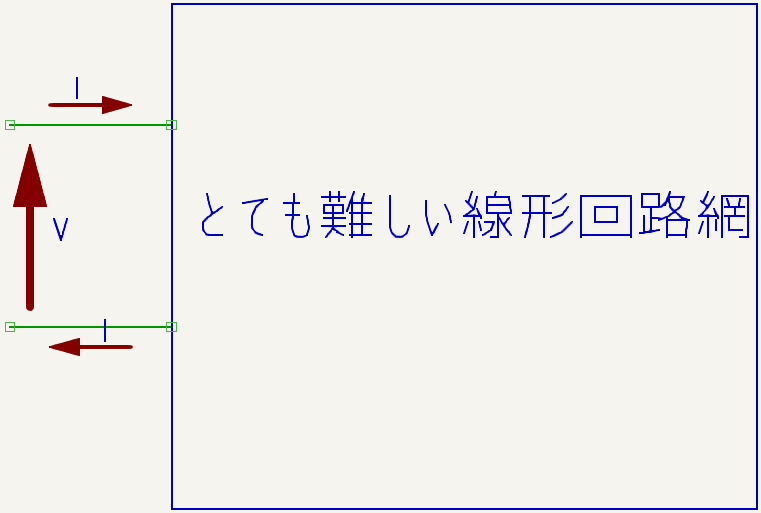
\includegraphics[width=0.5\textwidth]{circuit_theory/two_port_network.png}
    \caption{二端子対回路の概念図}
    \label{fig:two_port_network}
\end{figure}

このような二端子対に対して、電圧$V$と電流$I$の関係にのみ着目すれば、内部の複雑な回路構成を無視して、二端子対を一つの素子として扱うことができる。
\newpage
\subsection{入出力インピーダンス}

二端子対回路の考え方を応用したものとして、入力インピーダンスと出力インピーダンスの概念がある。

ある回路網の二端子対に交流信号を印加したとき、その二端子対に流れる電流($I$)と電圧($V$)に対して、入力インピーダンスとは、
\begin{align}
    Z_{in} = \frac{V}{I}
\end{align}
で定義される。
このとき、二端子対回路は、交流信号源から見たときに、抵抗値$Z_{in}$を持つ素子として振る舞うことになる。(図\ref{fig:input_impedance}参照)
\begin{figure}[htbp]
    \centering
    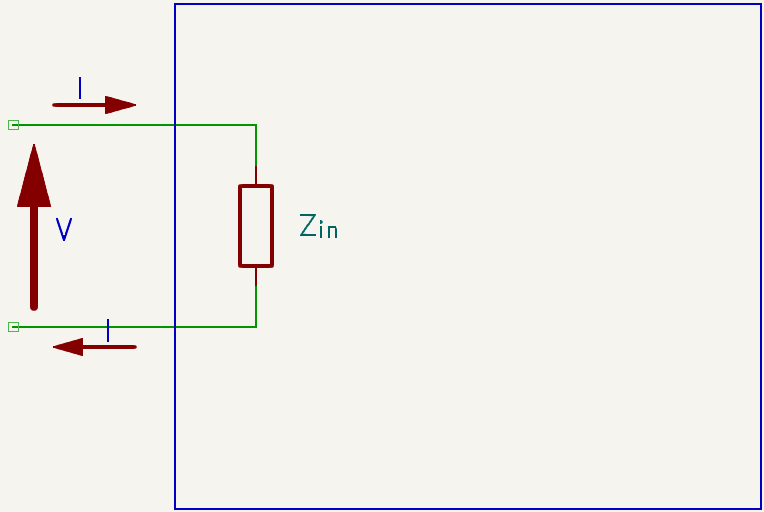
\includegraphics[width=0.5\textwidth]{circuit_theory/input_impedance.png}
    \caption{入力インピーダンスの概念図}
    \label{fig:input_impedance}
\end{figure}

同様に、ある回路網が電源として、二端子に電力を供給しているとき、起電力$E$と出力インピーダンス$Z_{out}$は、図\ref{fig:output_impedance}のように表される。
\begin{figure}[htbp]
    \centering
    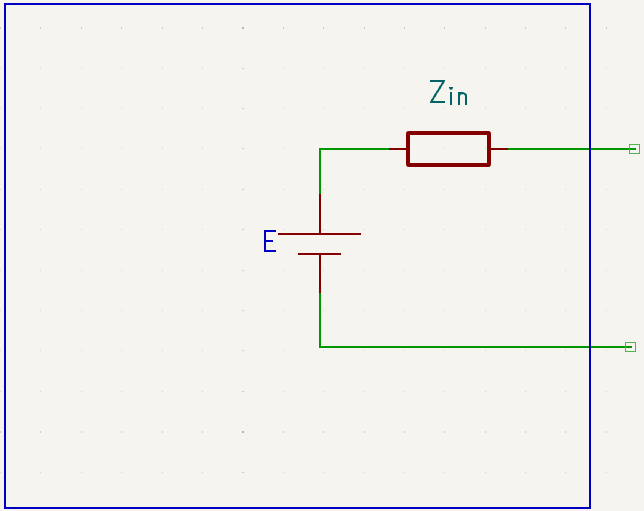
\includegraphics[width=0.5\textwidth]{circuit_theory/output_impedance.png}
    \caption{出力インピーダンスの概念図}
    \label{fig:output_impedance}
\end{figure}

入力インピーダンスは素子の入力側から見た特性を表し、高いほど電流を消費しないため良いとされている。
一方、出力インピーダンスは素子の出力側から見た特性を表し、低いほど負荷に対して安定した電圧を供給できるため良いとされている。
